\documentclass[t]{beamer}
\usetheme{Copenhagen}
\setbeamertemplate{headline}{} % remove toc from headers
\beamertemplatenavigationsymbolsempty

\usepackage{amsmath, array, tikz, bm, pgfplots, tcolorbox, tkz-euclide}
\usetkzobj{all}
\pgfplotsset{compat = 1.16}

\title{Patterns and Inductive Reasoning}
\author{}
\date{}

% \begin{tcolorbox}[colframe=green!20!black, colback = green!30!white,title=\textbf{TITLE}]

\AtBeginSection[]
{
  \begin{frame}
    \frametitle{Objectives}
    \tableofcontents[currentsection]
  \end{frame}
}

\begin{document}

\begin{frame} 
\maketitle
\end{frame}

\section{Use inductive reasoning to find the next terms of a pattern}

\begin{frame}{Inductive Reasoning}
\begin{tcolorbox}[colframe=green!20!black, colback = green!30!white,title=\textbf{Inductive Reasoning}]
\textbf{Inductive Reasoning} is reasoning that is based on some pattern observed.
\end{tcolorbox}
\end{frame}

\begin{frame}{Example 1}
Look for a pattern. What are the next 2 terms in each sequence?	\newline\\
(a)	\quad 3, 9, 27, 81, ...   \newline\\	\pause
Multiply by 3 to get each new term.	\newline\\	\pause
81(3) = 243	\newline\\	\pause
243(3) = 729	\newline\\	\pause
The next two terms are 243 and 729.
\end{frame}

\begin{frame}{Example 1}
(b)	\newline\\
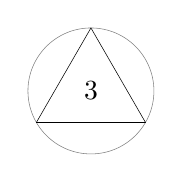
\begin{tikzpicture}[scale=0.8]
    \tkzDefPoints{0/0/A}
    \tkzDefShiftPoint[A](-30:1){B}
    \tkzDefShiftPoint[A](90:1){C}
    \tkzDefShiftPoint[A](210:1){D}
    \tkzDrawCircle(A,B)
    \tkzDrawSegments(B,C C,D D,B)
    \onslide<2->{\node at (A) {3};}
\end{tikzpicture}
\hspace{0.25in}
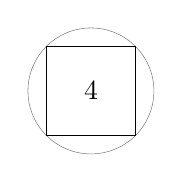
\begin{tikzpicture}[scale=0.8]
    \tkzDefPoints{0/0/A}
    \tkzDefShiftPoint[A](-45:1){B}
    \tkzDefShiftPoint[A](45:1){C}
    \tkzDefShiftPoint[A](135:1){D}
    \tkzDefShiftPoint[A](225:1){E}
    \tkzDrawCircle(A,B)
    \tkzDrawSegments(B,C C,D D,E E,B)
    \onslide<2->{\node at (A) {4};}
\end{tikzpicture}
\hspace{0.25in}
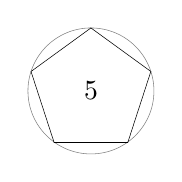
\begin{tikzpicture}[scale=0.8]
    \tkzDefPoints{0/0/A}
    \tkzDefShiftPoint[A](90:1){B}
    \tkzDefShiftPoint[A](162:1){C}
    \tkzDefShiftPoint[A](234:1){D}
    \tkzDefShiftPoint[A](306:1){E}
    \tkzDefShiftPoint[A](378:1){F}
    \tkzDefShiftPoint[A](450:1){G}
    \tkzDrawCircle(A,B)
    \tkzDrawSegments(B,C C,D D,E E,F F,G)
    \onslide<2->{\node at (A) {5};}
\end{tikzpicture}
\newline\\	

\onslide<3->{Each has a circle and number of sides increases by 1 each time.}	\newline\\
\onslide<4->{
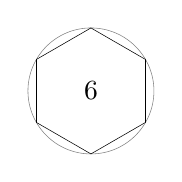
\begin{tikzpicture}[scale=0.8]
    \tkzDefPoints{0/0/A}
    \tkzDefShiftPoint[A](90:1){B}
    \tkzDefShiftPoint[A](150:1){C}
    \tkzDefShiftPoint[A](210:1){D}
    \tkzDefShiftPoint[A](270:1){E}
    \tkzDefShiftPoint[A](330:1){F}
    \tkzDefShiftPoint[A](30:1){G}
    \tkzDrawCircle(A,B)
    \tkzDrawSegments(B,C C,D D,E E,F F,G G,B)
    \node at (A) {6};
\end{tikzpicture}}
\hspace{0.25in}
\onslide<5->{
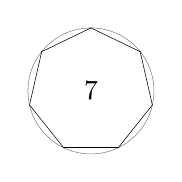
\begin{tikzpicture}[scale=0.8]
    \tkzDefPoints{0/0/A}
    \tkzDefShiftPoint[A](90:1){B}
    \tkzDefShiftPoint[A](141.43:1){C}
    \tkzDefShiftPoint[A](192.86:1){D}
    \tkzDefShiftPoint[A](244.29:1){E}
    \tkzDefShiftPoint[A](295.71:1){F}
    \tkzDefShiftPoint[A](347.14:1){G}
    \tkzDefShiftPoint[A](38.57:1){H}
    \tkzDrawCircle(A,B)
    \tkzDrawSegments(B,C C,D D,E E,F F,G G,H H,B)
    \node at (A) {7};
\end{tikzpicture}}
\end{frame}

\begin{frame}{Conjectures}
\begin{tcolorbox}[colframe=green!20!black, colback = green!30!white,title=\textbf{Conjectures}]
A \textbf{conjecture} is a conclusion you reach based on inductive reasoning.
\end{tcolorbox}
\end{frame}

\begin{frame}{Example 2}
Look at the circles. What conjecture can you make about the number of regions 20 diameters form?	\newline\\
\begin{center}
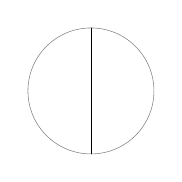
\begin{tikzpicture}[scale=0.8]
    \tkzDefPoints{0/0/A, 1/0/B, 0/1/C, 0/-1/D}
    \tkzDrawCircle(A,B)
    \tkzDrawSegment(C,D)
\end{tikzpicture}
\hspace{0.25in}
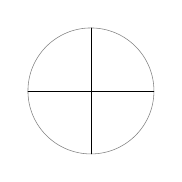
\begin{tikzpicture}[scale=0.8]
    \tkzDefPoints{0/0/A, 1/0/B, 0/1/C, 0/-1/D, -1/0/E}
    \tkzDrawCircle(A,B)
    \tkzDrawSegments(C,D B,E)
\end{tikzpicture}
\hspace{0.25in}
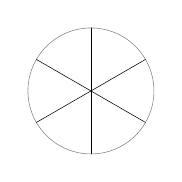
\begin{tikzpicture}[scale=0.8]
    \tkzDefPoints{0/0/A, 1/0/Z}
    \tkzDrawCircle(A,Z)
    \tkzDefShiftPoint[A](30:1){B}
    \tkzDefShiftPoint[A](90:1){C}
    \tkzDefShiftPoint[A](150:1){D}
    \tkzDefShiftPoint[A](210:1){E}
    \tkzDefShiftPoint[A](270:1){F}
    \tkzDefShiftPoint[A](330:1){G}
    \tkzDrawSegments(B,E C,F D,G)
\end{tikzpicture}
\newline\\
\onslide<2->{
	\begin{tabular}{|c|c|c|c|c|c|}
	\textbf{Num diam} & 1 & 2 & 3 & $\dots$ & 20 \\ \hline
	\textbf{Num regions} & 2 & 4 & 6 & $\dots$ & \onslide<4->{\textbf{40}} \\
	\end{tabular}	\newline\\
}
\onslide<3->{Num regions = 2 $\times$ num diameters}
\end{center}
\end{frame}

\begin{frame}{Example 3}
What conjecture can you make about the sum of the first 30 even numbers?
\end{frame}
\end{document}